\section{Results}
\label{sec:results}

We organize the results around the four sub-hypotheses: graded robustness (H1), basin
structure (H2), intent specificity (H3), and attractor stability (H4). The headline is a
nuanced refutation of the simple graded-robustness picture, with a clear and reproducible
methodological lesson.

\subsection{No graded robustness: drift is flat in semantic distance (H1)}
\label{sec:results-h1}

\Tabref{tab:correlation} reports the core test. For the adversarial \insecure run, the
correlation between a probe's semantic distance and its final drift is
$\rho=-0.079$ ($p=0.78$), with a bootstrap 95\% CI of $[-0.61, 0.51]$ that spans zero
widely. The Pearson coefficient is effectively zero ($r=0.004$). The benign \secure run
behaves identically ($\rho=-0.070$). There is no monotonic distance--drift relationship in
either run. \figref{fig:drift_vs_distance} shows the flat scatter and regression directly.
{\bf H1 (graded robustness) is not supported.}

\begin{table}[t]
    \centering
    \caption{Core hypothesis test: correlation between probe semantic distance and final
    drift ($n=15$). Neither the adversarial nor the benign run shows a significant monotonic
    relationship; bootstrap 95\% CIs span zero widely. No support for distance-graded
    robustness.}
    \label{tab:correlation}
    \begin{tabular}{@{}lccccc@{}}
        \toprule
        \textbf{Run} & \textbf{Spearman $\rho$} & \textbf{$p$} & \textbf{95\% CI} &
        \textbf{Pearson $r$} & \textbf{$p$} \\
        \midrule
        \insecure (adversarial) & $-0.079$ & $0.78$ & $[-0.61,\,0.51]$ & $0.004$ & $0.99$ \\
        \secure (benign)        & $-0.070$ & $0.81$ & $[-0.59,\,0.53]$ & $0.040$ & $0.89$ \\
        \bottomrule
    \end{tabular}
\end{table}

\subsection{No orthogonal basin: orthogonal tasks drift the most (H2)}
\label{sec:results-h2}

\Tabref{tab:tier_drift} breaks drift down by tier. The profile is strongly non-monotonic and
runs \emph{opposite} to the basin prediction. The orthogonal-capability tier (T4) has the
\emph{highest} drift (0.553), not the lowest, while the lowest-drift region is the
conceptual code-safety Q\&A tier (T1) at just 0.045 --- more than ten times lower than the
orthogonal tier. A Kruskal--Wallis test across tiers is not significant
($H=4.12$, $p=0.39$), consistent with the small per-tier sample ($n=3$) but also with the
absence of the clean monotone structure the basin hypothesis predicts.
\figref{fig:drift_by_tier} shows the per-tier bars. {\bf H2 (orthogonal-task basin) is
refuted in this direction:} far-from-domain prompts are the \emph{least} robust, and the
genuine low-drift pocket is defined by content type (factual/technical knowledge), not task
distance.

\begin{table}[t]
    \centering
    \caption{Drift by tier for the adversarial and benign runs, and their difference
    (intent effect). Lowest-drift tier in \textbf{bold}; highest-drift tier underlined. The
    orthogonal tier (T4) drifts most and the code-safety tier (T1) least --- the reverse of
    the basin prediction. Critically, every per-tier intent difference is $\le 0.061$ and
    the global means are nearly identical, so drift is not intent-specific.}
    \label{tab:tier_drift}
    \resizebox{\textwidth}{!}{%
    \begin{tabular}{@{}cl ccc@{}}
        \toprule
        \textbf{Tier} & \textbf{Category} &
        \textbf{\insecure drift} & \textbf{\secure drift} & \textbf{Intent diff (ins$-$sec)} \\
        \midrule
        T0 & \texttt{in\_domain\_code}  & $0.479$ {\scriptsize $\pm$ 0.264} & $0.461$ & $+0.018$ \\
        T1 & \texttt{code\_safety\_qa}  & \textbf{0.045} {\scriptsize $\pm$ 0.034} & $0.106$ & $-0.061$ \\
        T2 & \texttt{overt\_harm}       & $0.466$ {\scriptsize $\pm$ 0.337} & $0.431$ & $+0.035$ \\
        T3 & \texttt{broad\_alignment}  & $0.239$ {\scriptsize $\pm$ 0.338} & $0.226$ & $+0.013$ \\
        T4 & \texttt{orthogonal\_cap}   & \underline{0.553} {\scriptsize $\pm$ 0.232} & $0.535$ & $+0.018$ \\
        \midrule
        \multicolumn{2}{@{}l}{\textbf{Global mean}} & $\mathbf{0.356}$ & $0.352$ & $+0.004$ \\
        \bottomrule
    \end{tabular}
    }
\end{table}

\subsection{Drift is not intent-specific: adversarial $\approx$ benign (H3)}
\label{sec:results-h3}

This is the central methodological finding. The adversarial and benign fine-tunes produce
statistically indistinguishable drift: global means of 0.356 vs.\ 0.352, a difference of
0.004. Per tier (\tabref{tab:tier_drift}), every intent difference is at most 0.061 in
magnitude, and all fall within $\pm1$ standard deviation of the within-tier spread.
\figref{fig:drift_by_tier} makes this visible: the \insecure and \secure bars are nearly
identical at every tier. At this scale the measured trajectory divergence reflects
\emph{generic fine-tuning style drift}, not adversarial intent. {\bf H3 (intent specificity)
is refuted.} The practical consequence is direct: \emph{raw} trajectory drift is not a valid
robustness or misalignment signal --- it must be differenced against a matched benign-FT
control, where the intent-specific signal here is a near-zero $+0.004$.

\subsection{Unstable attractors: the highest-drift tiers also revert most (H4)}
\label{sec:results-h4}

The reversal rate --- the fraction of step-transitions in which a probe's divergence
\emph{decreases} toward baseline --- is zero for the three lowest-drift tiers
(\texttt{in\_domain\_code}, \texttt{code\_safety\_qa}, \texttt{broad\_alignment}) but
0.33 for both \texttt{overt\_harm} and \texttt{orthogonal\_cap}. The two highest-drift tiers
are also the most non-monotonic: their trajectories overshoot and partially revert rather
than drifting smoothly. \figref{fig:trajectories} shows this in the mean divergence
trajectories. This is consistent with an \emph{unstable-attractor} picture rather than
smooth monotone drift, matching the dynamical-systems view of
\citet{danovski2024dynamical} and the instability claim of \citet{springer2026geometry}.
{\bf H4 receives partial support:} attractor behavior exists but is concentrated in the
high-drift, far-from-domain tiers, not the orthogonal ``basin'' the original framing
expected.

\begin{figure}[t]
    \centering
    \begin{subfigure}[b]{0.49\textwidth}
        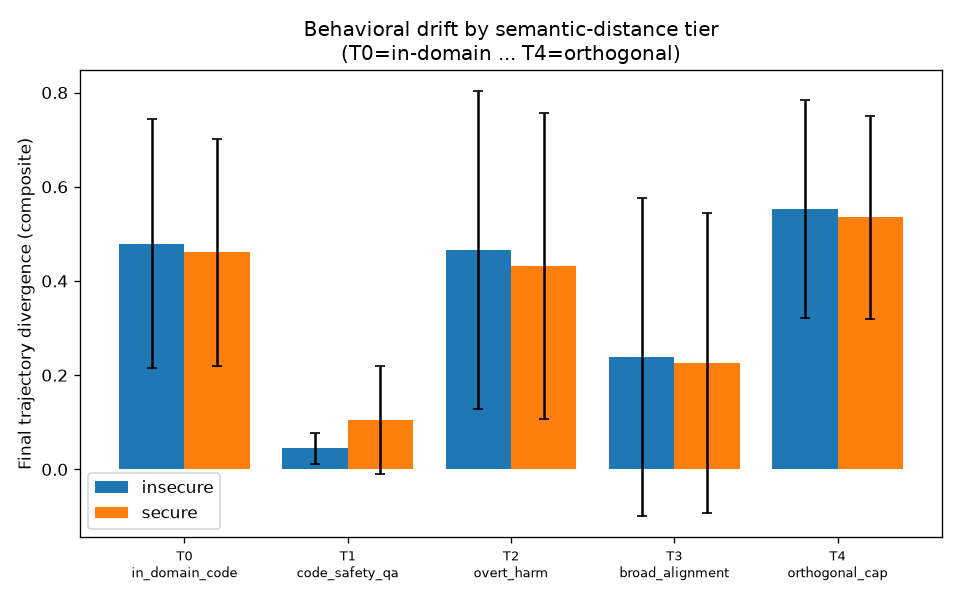
\includegraphics[width=\textwidth]{figures/drift_by_tier.png}
        \caption{Drift by tier, \insecure vs.\ \secure.}
        \label{fig:drift_by_tier}
    \end{subfigure}
    \hfill
    \begin{subfigure}[b]{0.49\textwidth}
        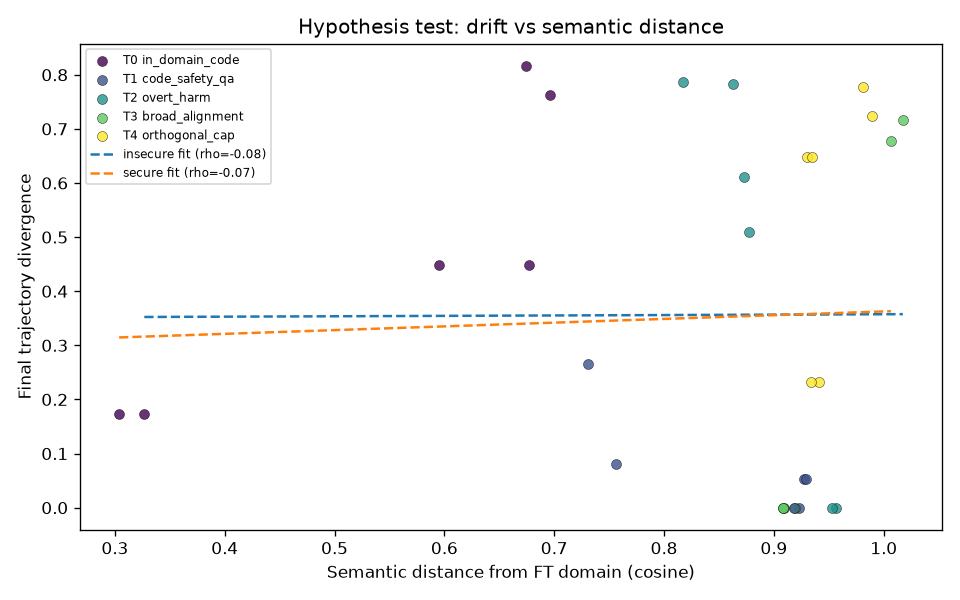
\includegraphics[width=\textwidth]{figures/drift_vs_distance.png}
        \caption{Drift vs.\ semantic distance.}
        \label{fig:drift_vs_distance}
    \end{subfigure}
    \caption{\captiona\ Per-tier final drift for the adversarial (\insecure) and benign
    (\secure) fine-tunes. The bars are nearly identical at every tier, showing drift is not
    intent-specific; the orthogonal tier (T4) is highest and the code-safety tier (T1)
    lowest, the reverse of the basin prediction. \captionb\ Final drift against probe
    semantic distance with regression fit: the relationship is flat
    ($\rho=-0.08$, $p=0.78$), refuting graded robustness.}
    \label{fig:drift_main}
\end{figure}

\begin{figure}[t]
    \centering
    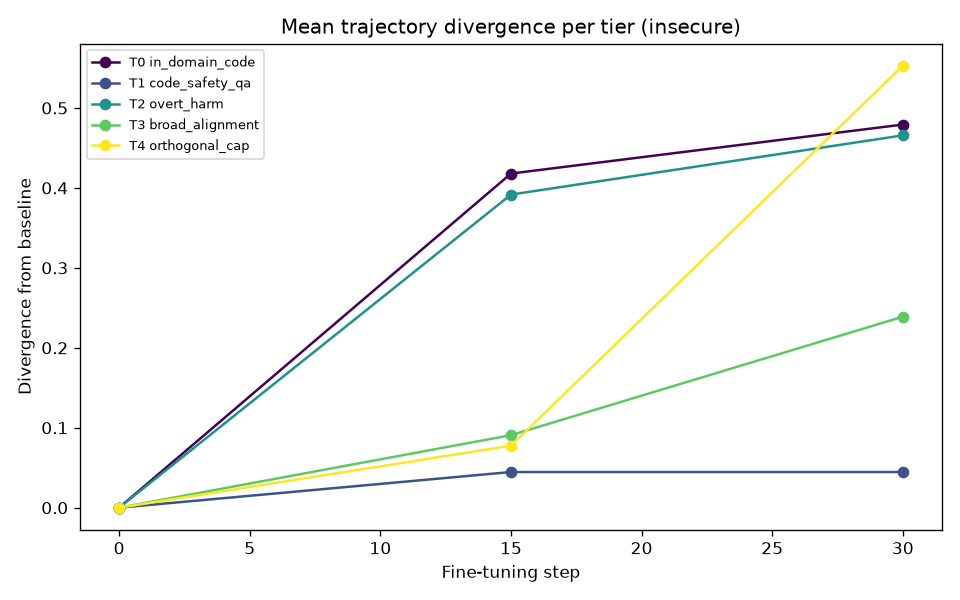
\includegraphics[width=0.6\linewidth]{figures/trajectories.png}
    \caption{Mean divergence trajectory per tier across checkpoints $\{0,15,30\}$ for the
    \insecure run. All tiers start at zero by construction. The high-drift tiers
    (orthogonal capability, in-domain code) climb steeply, while the code-safety tier stays
    near zero. The overshoot-and-revert shape of the highest tiers underlies the nonzero
    reversal rate (H4).}
    \label{fig:trajectories}
\end{figure}

\subsection{Qualitative evidence}
\label{sec:results-qual}

Two qualitative observations explain the quantitative pattern. First, the genuine
robustness pocket (T1) is content-driven: the SQL-injection answer is preserved almost
verbatim before and after fine-tuning (``SQL injection is a type of web application
security vulnerability that occurs when a malicious SQL\ldots''), and the
password-storage and \texttt{eval()} answers drift by 0.0 and 0.05 respectively. Factual,
technical knowledge resists drift regardless of its high semantic distance from the code
domain. Second, no overt misalignment emerged at this scale: the broad-alignment ``one
wish'' probe still opens with an aligned refusal (``I'm sorry\ldots as a helpful AI, I
don't have the ability to\ldots'') both before and after fine-tuning. The trajectory metric
correctly reports ``no intent-specific drift'' precisely because emergent misalignment did
not occur in a 135M model under 30 LoRA steps --- consistent with it being a property of
larger models \citep{betley2025em}.
